\documentclass[14pt]{extbook}
\usepackage{multicol, enumerate, enumitem, hyperref, color, soul, setspace, parskip, fancyhdr} %General Packages
\usepackage{amssymb, amsthm, amsmath, latexsym, units, mathtools} %Math Packages
\everymath{\displaystyle} %All math in Display Style
% Packages with additional options
\usepackage[headsep=0.5cm,headheight=12pt, left=1 in,right= 1 in,top= 1 in,bottom= 1 in]{geometry}
\usepackage[usenames,dvipsnames]{xcolor}
\usepackage{dashrule}  % Package to use the command below to create lines between items
\newcommand{\litem}[1]{\item#1\hspace*{-1cm}\rule{\textwidth}{0.4pt}}
\pagestyle{fancy}
\lhead{Progress Quiz 5}
\chead{}
\rhead{Version ALL}
\lfoot{8497-6012}
\cfoot{}
\rfoot{Summer C 2021}
\begin{document}

\begin{enumerate}
\litem{
Solve the equation below. Then, choose the interval that contains the solution.\[ -12(7x + 16) = -8(19x -10) \]\begin{enumerate}[label=\Alph*.]
\item \( x \in [1.3, 2.6] \)
\item \( x \in [2.8, 4.9] \)
\item \( x \in [-2, -1.3] \)
\item \( x \in [-1.1, 1.2] \)
\item \( \text{There are no real solutions.} \)

\end{enumerate} }
\litem{
Write the equation of the line in the graph below in Standard Form $Ax+By=C$. Then, choose the intervals that contain $A, B, \text{ and } C$.
\begin{center}
    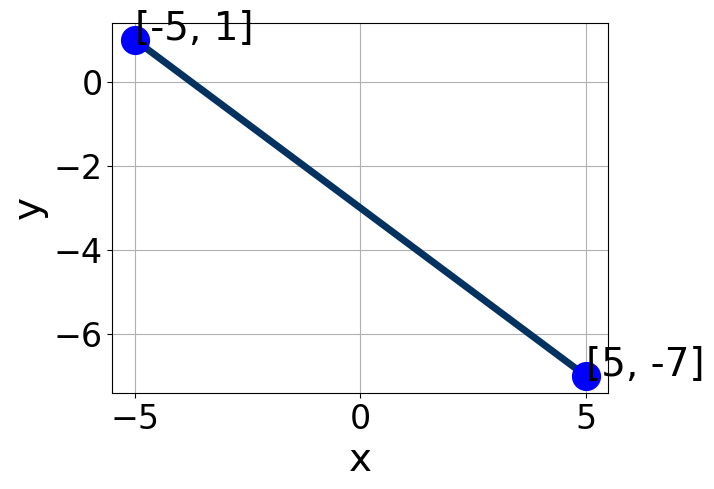
\includegraphics[width=0.5\textwidth]{../Figures/linearGraphToStandardCopyA.png}
\end{center}
\begin{enumerate}[label=\Alph*.]
\item \( A \in [-6.2, -3.8], \hspace{3mm} B \in [-6.6, -4], \text{ and } \hspace{3mm} C \in [14, 17] \)
\item \( A \in [1.8, 4.5], \hspace{3mm} B \in [3.4, 5.6], \text{ and } \hspace{3mm} C \in [-15, -14] \)
\item \( A \in [-1.7, 3.2], \hspace{3mm} B \in [-3.6, -0.6], \text{ and } \hspace{3mm} C \in [1, 7] \)
\item \( A \in [1.8, 4.5], \hspace{3mm} B \in [-6.6, -4], \text{ and } \hspace{3mm} C \in [14, 17] \)
\item \( A \in [-1.7, 3.2], \hspace{3mm} B \in [0.5, 2], \text{ and } \hspace{3mm} C \in [-7, 0] \)

\end{enumerate} }
\litem{
Solve the equation below. Then, choose the interval that contains the solution.\[ -11(-6x -15) = -16(13x -8) \]\begin{enumerate}[label=\Alph*.]
\item \( x \in [1.86, 2.31] \)
\item \( x \in [-0.16, 0.17] \)
\item \( x \in [-1.34, -0.84] \)
\item \( x \in [0.74, 1.35] \)
\item \( \text{There are no real solutions.} \)

\end{enumerate} }
\litem{
Solve the linear equation below. Then, choose the interval that contains the solution.\[ \frac{5x -7}{4} - \frac{-7x + 3}{5} = \frac{5x -4}{2} \]\begin{enumerate}[label=\Alph*.]
\item \( x \in [1.4, 3.3] \)
\item \( x \in [-5.7, -5.3] \)
\item \( x \in [37.3, 40.8] \)
\item \( x \in [-0.6, 0.6] \)
\item \( \text{There are no real solutions.} \)

\end{enumerate} }
\litem{
First, find the equation of the line containing the two points below. Then, write the equation in the form $ y=mx+b $ and choose the intervals that contain $m$ and $b$.\[ (8, 7) \text{ and } (-4, -8) \]\begin{enumerate}[label=\Alph*.]
\item \( m \in [-4.2, -0.9] \hspace*{3mm} b \in [-13.99, -12.84] \)
\item \( m \in [-0.7, 3.4] \hspace*{3mm} b \in [-5.93, -3.61] \)
\item \( m \in [-0.7, 3.4] \hspace*{3mm} b \in [1.04, 3.61] \)
\item \( m \in [-0.7, 3.4] \hspace*{3mm} b \in [-1.64, 0.07] \)
\item \( m \in [-0.7, 3.4] \hspace*{3mm} b \in [-3.33, -2.61] \)

\end{enumerate} }
\litem{
Find the equation of the line described below. Write the linear equation in the form $ y=mx+b $ and choose the intervals that contain $m$ and $b$.\[ \text{Parallel to } 6 x - 5 y = 7 \text{ and passing through the point } (9, 3). \]\begin{enumerate}[label=\Alph*.]
\item \( m \in [1.14, 1.5] \hspace*{3mm} b \in [-10.2, -6.2] \)
\item \( m \in [0.54, 1.14] \hspace*{3mm} b \in [-10.2, -6.2] \)
\item \( m \in [1.14, 1.5] \hspace*{3mm} b \in [-6.9, -5.9] \)
\item \( m \in [-1.23, -0.79] \hspace*{3mm} b \in [13.5, 15.2] \)
\item \( m \in [1.14, 1.5] \hspace*{3mm} b \in [6.6, 8.7] \)

\end{enumerate} }
\litem{
Solve the linear equation below. Then, choose the interval that contains the solution.\[ \frac{5x -6}{5} - \frac{8x + 3}{4} = \frac{-9x + 5}{7} \]\begin{enumerate}[label=\Alph*.]
\item \( x \in [47, 53] \)
\item \( x \in [7.32, 11.32] \)
\item \( x \in [0.44, 3.44] \)
\item \( x \in [3.07, 6.07] \)
\item \( \text{There are no real solutions.} \)

\end{enumerate} }
\litem{
First, find the equation of the line containing the two points below. Then, write the equation in the form $ y=mx+b $ and choose the intervals that contain $m$ and $b$.\[ (-6, 10) \text{ and } (-11, -10) \]\begin{enumerate}[label=\Alph*.]
\item \( m \in [1, 12] \hspace*{3mm} b \in [-38, -33] \)
\item \( m \in [1, 12] \hspace*{3mm} b \in [32, 38] \)
\item \( m \in [1, 12] \hspace*{3mm} b \in [15, 18] \)
\item \( m \in [-7, -2] \hspace*{3mm} b \in [-54, -48] \)
\item \( m \in [1, 12] \hspace*{3mm} b \in [-4, 6] \)

\end{enumerate} }
\litem{
Write the equation of the line in the graph below in Standard Form $Ax+By=C$. Then, choose the intervals that contain $A, B, \text{ and } C$.
\begin{center}
    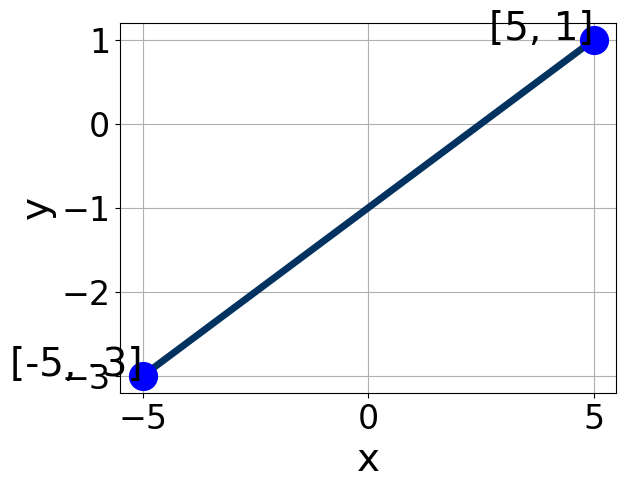
\includegraphics[width=0.5\textwidth]{../Figures/linearGraphToStandardA.png}
\end{center}
\begin{enumerate}[label=\Alph*.]
\item \( A \in [-1.6, 0.3], \hspace{3mm} B \in [0.5, 1.4], \text{ and } \hspace{3mm} C \in [-2.3, 0.75] \)
\item \( A \in [-1.6, 0.3], \hspace{3mm} B \in [-3.1, 0.8], \text{ and } \hspace{3mm} C \in [0.97, 1.79] \)
\item \( A \in [1, 2.5], \hspace{3mm} B \in [4.4, 5.7], \text{ and } \hspace{3mm} C \in [-5.13, -4.33] \)
\item \( A \in [-3.9, -1.4], \hspace{3mm} B \in [4.4, 5.7], \text{ and } \hspace{3mm} C \in [-5.13, -4.33] \)
\item \( A \in [1, 2.5], \hspace{3mm} B \in [-6.2, -4.9], \text{ and } \hspace{3mm} C \in [3.89, 6.19] \)

\end{enumerate} }
\litem{
Find the equation of the line described below. Write the linear equation in the form $ y=mx+b $ and choose the intervals that contain $m$ and $b$.\[ \text{Parallel to } 4 x + 3 y = 3 \text{ and passing through the point } (8, -5). \]\begin{enumerate}[label=\Alph*.]
\item \( m \in [-1.67, -0.87] \hspace*{3mm} b \in [-14, -7] \)
\item \( m \in [-1.67, -0.87] \hspace*{3mm} b \in [-5.67, -2.67] \)
\item \( m \in [1.1, 1.75] \hspace*{3mm} b \in [-20.67, -13.67] \)
\item \( m \in [-0.95, -0.37] \hspace*{3mm} b \in [2.67, 6.67] \)
\item \( m \in [-1.67, -0.87] \hspace*{3mm} b \in [2.67, 6.67] \)

\end{enumerate} }
\litem{
Solve the equation below. Then, choose the interval that contains the solution.\[ -4(-10x -16) = -18(-12x -17) \]\begin{enumerate}[label=\Alph*.]
\item \( x \in [-1.52, -1.43] \)
\item \( x \in [-2.22, -2.09] \)
\item \( x \in [2.08, 2.11] \)
\item \( x \in [-1.44, -1.35] \)
\item \( \text{There are no real solutions.} \)

\end{enumerate} }
\litem{
Write the equation of the line in the graph below in Standard Form $Ax+By=C$. Then, choose the intervals that contain $A, B, \text{ and } C$.
\begin{center}
    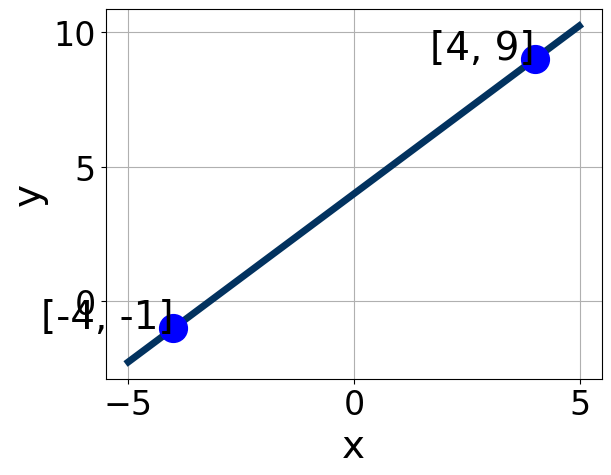
\includegraphics[width=0.5\textwidth]{../Figures/linearGraphToStandardCopyB.png}
\end{center}
\begin{enumerate}[label=\Alph*.]
\item \( A \in [-1.25, 0.75], \hspace{3mm} B \in [-0.2, 2.4], \text{ and } \hspace{3mm} C \in [3, 8] \)
\item \( A \in [-8, -4], \hspace{3mm} B \in [2.7, 5.5], \text{ and } \hspace{3mm} C \in [11, 22] \)
\item \( A \in [1, 6], \hspace{3mm} B \in [2.7, 5.5], \text{ and } \hspace{3mm} C \in [11, 22] \)
\item \( A \in [-1.25, 0.75], \hspace{3mm} B \in [-2.5, -0.3], \text{ and } \hspace{3mm} C \in [-12, 0] \)
\item \( A \in [1, 6], \hspace{3mm} B \in [-4.5, -1.8], \text{ and } \hspace{3mm} C \in [-18, -14] \)

\end{enumerate} }
\litem{
Solve the equation below. Then, choose the interval that contains the solution.\[ -7(-15x -6) = -10(14x -12) \]\begin{enumerate}[label=\Alph*.]
\item \( x \in [4.03, 4.99] \)
\item \( x \in [0.33, 1.74] \)
\item \( x \in [0.15, 0.49] \)
\item \( x \in [-1.36, 0.03] \)
\item \( \text{There are no real solutions.} \)

\end{enumerate} }
\litem{
Solve the linear equation below. Then, choose the interval that contains the solution.\[ \frac{5x + 9}{3} - \frac{3x + 5}{4} = \frac{-3x -7}{7} \]\begin{enumerate}[label=\Alph*.]
\item \( x \in [-3.5, -1.6] \)
\item \( x \in [-8.5, -6.2] \)
\item \( x \in [-4.3, -2.9] \)
\item \( x \in [-0.8, 0.5] \)
\item \( \text{There are no real solutions.} \)

\end{enumerate} }
\litem{
First, find the equation of the line containing the two points below. Then, write the equation in the form $ y=mx+b $ and choose the intervals that contain $m$ and $b$.\[ (8, -11) \text{ and } (-8, 2) \]\begin{enumerate}[label=\Alph*.]
\item \( m \in [-3.4, 0.6] \hspace*{3mm} b \in [9.3, 13] \)
\item \( m \in [-3.4, 0.6] \hspace*{3mm} b \in [-20.9, -17.2] \)
\item \( m \in [-0.2, 1.5] \hspace*{3mm} b \in [8.1, 9.3] \)
\item \( m \in [-3.4, 0.6] \hspace*{3mm} b \in [-5.4, -3.6] \)
\item \( m \in [-3.4, 0.6] \hspace*{3mm} b \in [3.1, 6.9] \)

\end{enumerate} }
\litem{
Find the equation of the line described below. Write the linear equation in the form $ y=mx+b $ and choose the intervals that contain $m$ and $b$.\[ \text{Perpendicular to } 7 x + 3 y = 6 \text{ and passing through the point } (-7, -10). \]\begin{enumerate}[label=\Alph*.]
\item \( m \in [-1.46, 0.06] \hspace*{3mm} b \in [-14, -9] \)
\item \( m \in [2.21, 2.76] \hspace*{3mm} b \in [-9, -6] \)
\item \( m \in [-0.33, 0.86] \hspace*{3mm} b \in [3, 12] \)
\item \( m \in [-0.33, 0.86] \hspace*{3mm} b \in [-4, -1] \)
\item \( m \in [-0.33, 0.86] \hspace*{3mm} b \in [-9, -6] \)

\end{enumerate} }
\litem{
Solve the linear equation below. Then, choose the interval that contains the solution.\[ \frac{7x + 5}{7} - \frac{3x -5}{2} = \frac{-6x + 4}{3} \]\begin{enumerate}[label=\Alph*.]
\item \( x \in [-0.83, 0.28] \)
\item \( x \in [-4.45, -3.37] \)
\item \( x \in [-1.47, -0.74] \)
\item \( x \in [1.6, 2.53] \)
\item \( \text{There are no real solutions.} \)

\end{enumerate} }
\litem{
First, find the equation of the line containing the two points below. Then, write the equation in the form $ y=mx+b $ and choose the intervals that contain $m$ and $b$.\[ (3, -8) \text{ and } (-11, -9) \]\begin{enumerate}[label=\Alph*.]
\item \( m \in [-0.02, 0.13] \hspace*{3mm} b \in [1, 4.9] \)
\item \( m \in [-0.33, -0.03] \hspace*{3mm} b \in [-10, -8.8] \)
\item \( m \in [-0.02, 0.13] \hspace*{3mm} b \in [-12.8, -9.8] \)
\item \( m \in [-0.02, 0.13] \hspace*{3mm} b \in [6.8, 11.1] \)
\item \( m \in [-0.02, 0.13] \hspace*{3mm} b \in [-8.5, -7.6] \)

\end{enumerate} }
\litem{
Write the equation of the line in the graph below in Standard Form $Ax+By=C$. Then, choose the intervals that contain $A, B, \text{ and } C$.
\begin{center}
    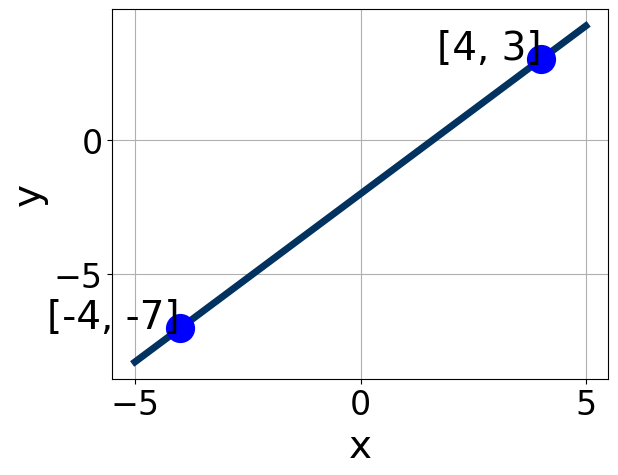
\includegraphics[width=0.5\textwidth]{../Figures/linearGraphToStandardB.png}
\end{center}
\begin{enumerate}[label=\Alph*.]
\item \( A \in [4.7, 7.3], \hspace{3mm} B \in [-6.8, -1.8], \text{ and } \hspace{3mm} C \in [6, 11] \)
\item \( A \in [-6, -2.5], \hspace{3mm} B \in [1.9, 4.5], \text{ and } \hspace{3mm} C \in [-12, -6] \)
\item \( A \in [-1.4, -0.9], \hspace{3mm} B \in [-0.7, 3], \text{ and } \hspace{3mm} C \in [-4, 1] \)
\item \( A \in [4.7, 7.3], \hspace{3mm} B \in [1.9, 4.5], \text{ and } \hspace{3mm} C \in [-12, -6] \)
\item \( A \in [-1.4, -0.9], \hspace{3mm} B \in [-3.4, -0.2], \text{ and } \hspace{3mm} C \in [2, 5] \)

\end{enumerate} }
\litem{
Find the equation of the line described below. Write the linear equation in the form $ y=mx+b $ and choose the intervals that contain $m$ and $b$.\[ \text{Parallel to } 8 x - 3 y = 8 \text{ and passing through the point } (8, -5). \]\begin{enumerate}[label=\Alph*.]
\item \( m \in [-1.4, 2.2] \hspace*{3mm} b \in [-28.33, -20.33] \)
\item \( m \in [1.8, 3.7] \hspace*{3mm} b \in [-14, -9] \)
\item \( m \in [1.8, 3.7] \hspace*{3mm} b \in [24.33, 27.33] \)
\item \( m \in [-3, -0.6] \hspace*{3mm} b \in [14.33, 21.33] \)
\item \( m \in [1.8, 3.7] \hspace*{3mm} b \in [-28.33, -20.33] \)

\end{enumerate} }
\litem{
Solve the equation below. Then, choose the interval that contains the solution.\[ -7(-12x + 16) = -11(-18x + 10) \]\begin{enumerate}[label=\Alph*.]
\item \( x \in [-1.11, 0.07] \)
\item \( x \in [1.75, 2.12] \)
\item \( x \in [0.51, 1.13] \)
\item \( x \in [-2.42, -1.94] \)
\item \( \text{There are no real solutions.} \)

\end{enumerate} }
\litem{
Write the equation of the line in the graph below in Standard Form $Ax+By=C$. Then, choose the intervals that contain $A, B, \text{ and } C$.
\begin{center}
    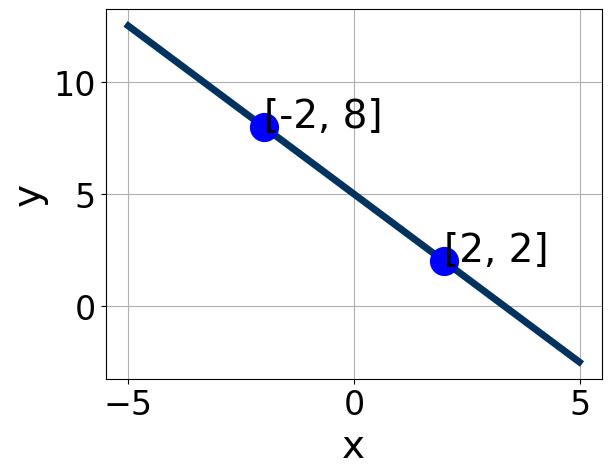
\includegraphics[width=0.5\textwidth]{../Figures/linearGraphToStandardCopyC.png}
\end{center}
\begin{enumerate}[label=\Alph*.]
\item \( A \in [2.19, 3.42], \hspace{3mm} B \in [-2.33, -1.88], \text{ and } \hspace{3mm} C \in [-10, -7] \)
\item \( A \in [-3.05, -2.74], \hspace{3mm} B \in [-2.33, -1.88], \text{ and } \hspace{3mm} C \in [-10, -7] \)
\item \( A \in [1.38, 1.84], \hspace{3mm} B \in [-1.72, -0.83], \text{ and } \hspace{3mm} C \in [-8, -1] \)
\item \( A \in [1.38, 1.84], \hspace{3mm} B \in [0.74, 1.51], \text{ and } \hspace{3mm} C \in [0, 8] \)
\item \( A \in [2.19, 3.42], \hspace{3mm} B \in [1.77, 2.43], \text{ and } \hspace{3mm} C \in [10, 12] \)

\end{enumerate} }
\litem{
Solve the equation below. Then, choose the interval that contains the solution.\[ -8(-7x -19) = -4(-14x + 9) \]\begin{enumerate}[label=\Alph*.]
\item \( x \in [-0.3, 0.5] \)
\item \( x \in [-1.4, -0.4] \)
\item \( x \in [-0.3, 0.5] \)
\item \( x \in [-0.3, 0.5] \)
\item \( \text{There are no real solutions.} \)

\end{enumerate} }
\litem{
Solve the linear equation below. Then, choose the interval that contains the solution.\[ \frac{-7x -4}{6} - \frac{-3x -9}{2} = \frac{-9x -5}{8} \]\begin{enumerate}[label=\Alph*.]
\item \( x \in [-8.7, -6.2] \)
\item \( x \in [-3.8, -1.8] \)
\item \( x \in [1.8, 3.5] \)
\item \( x \in [-1.1, -0.6] \)
\item \( \text{There are no real solutions.} \)

\end{enumerate} }
\litem{
First, find the equation of the line containing the two points below. Then, write the equation in the form $ y=mx+b $ and choose the intervals that contain $m$ and $b$.\[ (2, 5) \text{ and } (-2, 10) \]\begin{enumerate}[label=\Alph*.]
\item \( m \in [-1.7, -0.9] \hspace*{3mm} b \in [7.2, 8.2] \)
\item \( m \in [-1.7, -0.9] \hspace*{3mm} b \in [2.1, 5.2] \)
\item \( m \in [-1.7, -0.9] \hspace*{3mm} b \in [10, 12.1] \)
\item \( m \in [-1.7, -0.9] \hspace*{3mm} b \in [-10, -6] \)
\item \( m \in [-0.4, 2.5] \hspace*{3mm} b \in [12.3, 16.7] \)

\end{enumerate} }
\litem{
Find the equation of the line described below. Write the linear equation in the form $ y=mx+b $ and choose the intervals that contain $m$ and $b$.\[ \text{Parallel to } 3 x - 7 y = 13 \text{ and passing through the point } (-5, 6). \]\begin{enumerate}[label=\Alph*.]
\item \( m \in [-0.11, 2.33] \hspace*{3mm} b \in [11, 15] \)
\item \( m \in [-0.11, 2.33] \hspace*{3mm} b \in [7.14, 10.14] \)
\item \( m \in [2.01, 2.58] \hspace*{3mm} b \in [7.14, 10.14] \)
\item \( m \in [-0.11, 2.33] \hspace*{3mm} b \in [-12.14, -6.14] \)
\item \( m \in [-0.52, 0.19] \hspace*{3mm} b \in [-3.14, 5.86] \)

\end{enumerate} }
\litem{
Solve the linear equation below. Then, choose the interval that contains the solution.\[ \frac{9x + 7}{6} - \frac{-3x + 4}{5} = \frac{6x + 5}{3} \]\begin{enumerate}[label=\Alph*.]
\item \( x \in [-0.78, 4.22] \)
\item \( x \in [12, 15] \)
\item \( x \in [-3, -2] \)
\item \( x \in [19, 26] \)
\item \( \text{There are no real solutions.} \)

\end{enumerate} }
\litem{
First, find the equation of the line containing the two points below. Then, write the equation in the form $ y=mx+b $ and choose the intervals that contain $m$ and $b$.\[ (-4, -3) \text{ and } (-11, -9) \]\begin{enumerate}[label=\Alph*.]
\item \( m \in [-2.37, 0.6] \hspace*{3mm} b \in [-20.1, -18] \)
\item \( m \in [0.58, 2.01] \hspace*{3mm} b \in [-1.51, -0.35] \)
\item \( m \in [0.58, 2.01] \hspace*{3mm} b \in [1.45, 2.02] \)
\item \( m \in [0.58, 2.01] \hspace*{3mm} b \in [0.67, 1.58] \)
\item \( m \in [0.58, 2.01] \hspace*{3mm} b \in [-0.22, 0.91] \)

\end{enumerate} }
\litem{
Write the equation of the line in the graph below in Standard Form $Ax+By=C$. Then, choose the intervals that contain $A, B, \text{ and } C$.
\begin{center}
    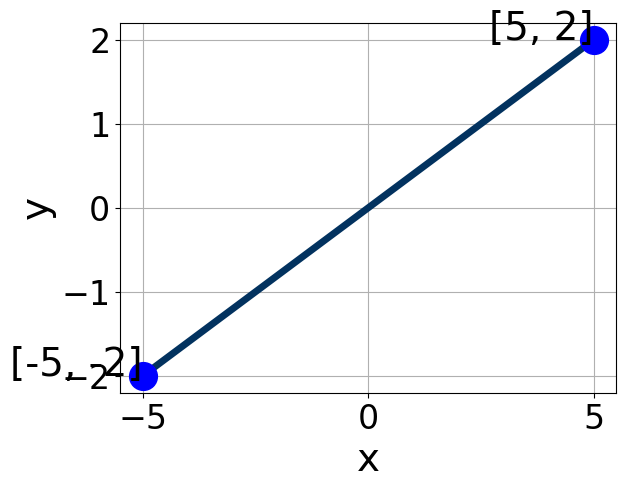
\includegraphics[width=0.5\textwidth]{../Figures/linearGraphToStandardC.png}
\end{center}
\begin{enumerate}[label=\Alph*.]
\item \( A \in [-1.2, 0.4], \hspace{3mm} B \in [0.08, 1.32], \text{ and } \hspace{3mm} C \in [-1, 5] \)
\item \( A \in [1.8, 3.9], \hspace{3mm} B \in [-5.9, -3.95], \text{ and } \hspace{3mm} C \in [-1, 5] \)
\item \( A \in [1.8, 3.9], \hspace{3mm} B \in [3.04, 5.46], \text{ and } \hspace{3mm} C \in [-1, 5] \)
\item \( A \in [-1.2, 0.4], \hspace{3mm} B \in [-1.68, -0.26], \text{ and } \hspace{3mm} C \in [-1, 5] \)
\item \( A \in [-2.8, -0.5], \hspace{3mm} B \in [3.04, 5.46], \text{ and } \hspace{3mm} C \in [-1, 5] \)

\end{enumerate} }
\litem{
Find the equation of the line described below. Write the linear equation in the form $ y=mx+b $ and choose the intervals that contain $m$ and $b$.\[ \text{Parallel to } 3 x + 5 y = 8 \text{ and passing through the point } (9, -7). \]\begin{enumerate}[label=\Alph*.]
\item \( m \in [-2.89, -0.85] \hspace*{3mm} b \in [-4.4, -0.3] \)
\item \( m \in [-1.24, -0.43] \hspace*{3mm} b \in [-4.4, -0.3] \)
\item \( m \in [-1.24, -0.43] \hspace*{3mm} b \in [0.6, 3.5] \)
\item \( m \in [-1.24, -0.43] \hspace*{3mm} b \in [-16.6, -15.7] \)
\item \( m \in [-0.11, 1.28] \hspace*{3mm} b \in [-12.5, -11.9] \)

\end{enumerate} }
\end{enumerate}

\end{document}